
\begin{frame}
  \maketitle
\end{frame}

\section{本編}
\begin{frame}{背景・目的}
  \begin{itemize}
  \item HPCにおけるネットワークのトポロジ(グラフ)
    \begin{itemize}
    \item 無向(スイッチは双方向に通信可能)
    \item 正則(すべてのスイッチは同一個数のポートを有する)
    \item 平均頂点間距離が短いと遅延も短い
      \cite{Koibuchi2012,Singla2011}
    \end{itemize}
  \end{itemize}
  \begin{columns}[T]
    \begin{column}{.5\textwidth}
      \begin{itemize}
      \item \alert{一般化ムーアグラフ}
        \begin{itemize}
        \item 平均頂点間距離が理論的な下界と等しい正則グラフ
          \cite{Cerf1973,Cerf1974Lower}
        \end{itemize}
      \item 一般化ムーアグラフを求める試み
        \cite{Yamamoto2016}
      \item 一般化ムーアグラフの性質を利用した探索法は知られていない
      \end{itemize}
    \end{column}
    \begin{column}{.5\textwidth}
      \begin{figure}
        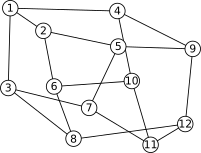
\includegraphics[width=.6\linewidth]{gmg-example}
        \caption{一般化ムーアグラフの例}
      \end{figure}
    \end{column}
  \end{columns}
  \begin{block}{}
    目的 : 一般化ムーアグラフの探索を効率的に行う方法の提案と評価
  \end{block}
\end{frame}

\begin{frame}[allowframebreaks]{探索アルゴリズム}
  \begin{columns}
    \begin{column}{.4\textwidth}
      \begin{figure}
        \centering
        \includegraphics[height=.3\textheight]{feasible-edges-example-color}
        \caption{初期グラフと候補辺}
      \end{figure}
    \end{column}
    \begin{column}{.6\textwidth}
      \small
      \par 深さ優先探索に基づく
      \begin{enumerate}
      \item 初期グラフから探索を開始する
      \item 候補辺を追加したグラフと追加しないグラフをスタックにプッシュする
      \item 定理\ref{thm:gmg-geom}の条件に反するならプッシュしない
      \end{enumerate}
    \end{column}
  \end{columns}
  \vspace*{-1em}
  \begin{theorem}
    \label{thm:gmg-geom}
    {\scriptsize
    正則グラフ$(n,k)$が一般化ムーアグラフであることの必要十分条件は
    次の二つの条件を同時に満たすことである.
    \begin{enumerate}
    \item 長さ$2Q$以下の閉路が存在しない.
      \label{itm:gmg-geom-1}
    \item $R=0$ならば直径が$Q$であり,$R>0$ならば直径が$Q+1$である.
      \label{itm:gmg-geom-2}
    \end{enumerate}
    \[ Q=\max\{q|n-1-\sum_{i=1}^{q}k(k-1)^{i-1}\geq 0\},\quad
    R=n-1-\sum_{i=1}^{Q}k(k-1)^{i-1} \]
    }
  \end{theorem}
\end{frame}

\begin{frame}{探索空間の削減}
  \begin{columns}[T]
    \begin{column}{.5\textwidth}
      \begin{itemize}
      \item 初期グラフの制限
      \end{itemize}
      \vspace*{-1em}
      \begin{figure}
        \centering
        \includegraphics[width=.7\columnwidth]
                        {initial-tree-cycle-example-color}
                        \caption{閉路を含むグラフ(閉路)}
      \end{figure}
      \vspace*{-2em}
      \begin{figure}
        \centering
        \includegraphics[width=.8\columnwidth]
                        {initial-spanning-tree-18-example-color}
                        \caption{全域木}
      \end{figure}
    \end{column}
    \begin{column}{.5\textwidth}
      \begin{itemize}
      \item 直径の下界を利用した枝刈り
      \item[] まだ見ていない候補辺をすべて追加したグラフの直径を計算
      \item[] 定理\ref{thm:gmg-geom}の条件\ref{itm:gmg-geom-2}に反するなら枝刈り
      \end{itemize}
      \begin{figure}
        \centering
        \includegraphics[width=.9\columnwidth]{max-graph-example-color}
        \caption{直径の下界の計算に用いるグラフ}
      \end{figure}
    \end{column}
  \end{columns}
\end{frame}

\begin{frame}{実験}
  \begin{itemize}
  \item 測定項目
    \begin{enumerate}
    \item 探索時間(10回の平均)
    \item 展開状態数(スタックからグラフを取り出した回数)
    \end{enumerate}
  \item パラメータ(頂点数$n$と次数$k$)
    \begin{itemize}
    \item[]\par$\begin{aligned}
      n &= 4,6,8,10,12,14,16,18 \\
      k &= 3
    \end{aligned}$
    \end{itemize}
  \item 実行環境
    \par\begin{table}
    \scriptsize
    \caption{実行環境}
    \label{tab:env-lab}
    \centering
    \begin{tabular}{ll}
      \hline
      プロセッサ & Intel® Core™ i5-4670 CPU @ 3.40GHz × 4 \\ \hline
      メインメモリ & 5.8GiB \\ \hline
      ゲストOS & Ubuntu 16.04.3 LTS 64 ビット \\ \hline
      仮想化 & Oracle VirtualBox バージョン 5.1.18 \\ \hline
      ホストOS & Windows 8.1 Pro 64 ビット \\ \hline
      コンパイラ & gcc 5.4.0 \\ \hline
      グラフライブラリ & igraph 0.7.1-2.1 \\ \hline
      最適化フラグ & -Ofast \\ \hline
    \end{tabular}
    \end{table}
  \end{itemize}
\end{frame}

\begin{frame}{結果}
  \begin{columns}[T]
    \begin{column}{.5\textwidth}
      \begin{itemize}
      \item 全域木を使うと最速で最も展開状態数が少ない
      \item 閉路は頂点数12で基本より展開状態数が多い
        \begin{itemize}
        \item 候補辺が適切な順番でなく,正則グラフの判定が遅くなるため
        \end{itemize}
        \medskip
      \item 枝刈りによって展開状態数が減少する
      \item 小さい頂点数に対して探索時間が増加する
        \begin{itemize}
        \item 下記により効率化が無効になるため
        \end{itemize}
        \vspace*{-.5em}
        \begin{enumerate}
        \item 直径の計算が必要になること
        \item 多くのグラフの生成と破棄が発生すること
        \end{enumerate}
      \end{itemize}
    \end{column}
    \begin{column}{.5\textwidth}
      \centering
      \includegraphics[height=.35\textheight]{cmp-algo-time}
      \captionof{figure}{平均探索時間}
      \vfill
      \includegraphics[height=.35\textheight]{cmp-algo-state}
      \captionof{figure}{展開状態数}
    \end{column}
  \end{columns}
\end{frame}

\begin{frame}{まとめ}
  \begin{itemize}
  \item 一般化ムーアグラフの探索の探索空間の削減の効果を研究
    \begin{itemize}
    \item 全域木
    \item 直径の下界を利用した枝刈り
    \end{itemize}
  \item[] を使用することで効率良く探索できる
  \item 今後の課題
    \begin{itemize}
    \item 提案した初期グラフへの制限の妥当性の検証
    \item 一般化ムーアグラフが存在しないときの平均頂点間距離最小のグラフ
    \end{itemize}
  \end{itemize}
  \begin{figure}
    \centering
    \includegraphics[width=\textwidth]{gmg-existence-h}
    \caption{発見した一般化ムーアグラフの頂点数と次数の組}
  \end{figure}
\end{frame}

\appendix
%\begin{frame}<handout:0>{付録}
%  ふろくです
%\end{frame}

\begin{frame}[allowframebreaks]{参考文献}
  \bibliography{../res/MyCollection}
\end{frame}


